\section{Library Configuration}
\label{sec.conf}

This section describes the conventions and assumptions made by
$\pvslm$ for managing PVS library sources.

\paragraph{Conventions.}
The $\pvslm$ tool distinguishes three levels of aggregation for PVS
sources. A PVS theory is the building block of a library managed by
$\pvslm$. A {\em package} is a collection of theories. At the top
level of aggregation is a {\em library}, which comprises a collection
of packages. Namely, a library is a collection of packages and a
package is a collection of libraries. The $\pvslm$ tool can manage
several libraries each with several packages. However, the tool does
not support management at the level of specific theory files.

\paragraph{Package configuration.}
Each package of a library is defined in a folder at the root of the
library source. The folder's name corresponds to the name of the
package. Each folder contains the corresponding \cde{pvs} and
\cde{prf} files for its theories, and the folder \cde{pvsbin}, a
special folder with the package's metadata described in a file named
\cde{top.dep}. Figure~\ref{fig.package} depicts the structure of
package \cde{analysis} from the NASA PVS Library~\cite{nasalib}
(NASALib).

\begin{figure}
  \centering
  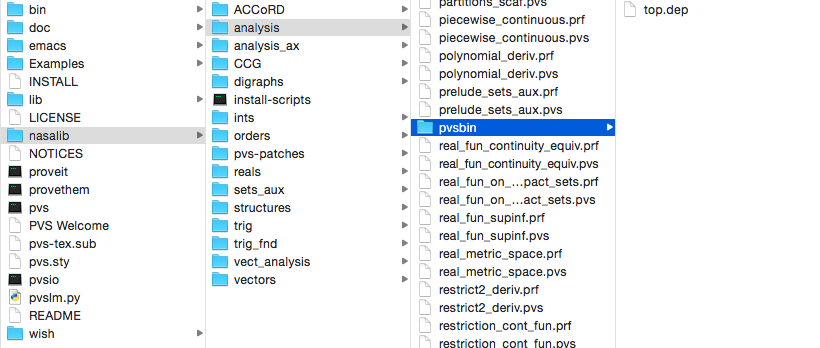
\includegraphics[width=11cm]{images/package.png}
  \caption{The structure of a package \cde{analysis}.}
  \label{fig.package}
\end{figure}

\paragraph{Package metadata.} The metadata of a package is defined
in its \cde{top.dep} file located inside folder
\cde{pvsbin}. Table~\ref{tab.bnf} presents the syntax of the metadata
file in BNF-like notation. The topmost symbol is
$\nterm{\cde{metadata}}$, while $\nterm{\cde{theory}}$ and
$\nterm{\cde{package}}$ are terminals representing, respectively,
theory and package names. The metadata comprises two parts, namely, a
header and a body. The header corresponds to a single line with an `/'
symbol followed by a comma-separated list of theory names; these names
correspond to the names of the theories included in the package (in
any order). A body comprises any number of lines, each with either a
package dependency or a theory dependency. A package dependency
describes a dependency from another package and the list of theories
from that external package being used. A theory dependency describes,
for each one of the theories listed in the header of the package, its
list of theory dependencies. In the case such a theory depends on a
theory from other package, the name of that dependency must be
qualified by the name of the corresponding package.

\begin{table}
  \centering
  \begin{tabular}{r c p{8cm}}
    \hline \\
    $\nterm{\cde{metadata}}$ & ::= & $\nterm{\cde{header}} \; \nterm{\cde{body}}$ \\
    $\nterm{\cde{header}}$ & ::= & `/' $\nterm{\cde{theorylist}}$ \\
    $\nterm{\cde{theorylist}}$ & ::= & $\nterm{\cde{theory}} \mid \nterm{\cde{theory}}$ `,' $\nterm{\cde{theorylist}}$ \\
    $\nterm{\cde{body}}$ & ::= & $(\nterm{\cde{packagedep}} \mid \nterm{\cde{theorydep}})*$ \\
    $\nterm{\cde{packagedep}}$ & ::= & $\nterm{\cde{package}}$ `/' $\nterm{\cde{theorylist}}$ \\
    $\nterm{\cde{theorydep}}$ & ::= & $\nterm{\cde{theory}}$ `:' $\nterm{\cde{qualtheorylist}} ?$ \\
    $\nterm{\cde{qualtheorylist}}$ & ::= & $\nterm{\cde{qualtheory}} \mid \nterm{\cde{qualtheory}}$ `,' $\nterm{\cde{qualtheorylist}}$ \\
    $\nterm{\cde{qualtheory}}$ & ::= & $(\nterm{\cde{package}}\; \text{`@'})?$ $\nterm{\cde{theory}}$ \\
    \\
    \hline
  \end{tabular}
  \caption{Syntax of the \cde{top.dep} metadata file.}
  \label{tab.bnf}
\end{table}

Figure~\ref{fig.top} presents an overview of the configuration file
for package \cde{trig} in NASALib. According to the header
description, package \cde{trig} defines theories \cde{top},
\cde{trig\_doc}, \cde{trig}, \cde{trig\_values}, etc. It contains $5$
package dependencies and $7$ theory dependencies. For instance,
package \cde{trig} depends on theory \cde{for\_iterate} from package
\cde{structures}, and on theories \cde{finite\_sets\_minmax} and
\cde{finite\_sets\_inductions} from package \cde{finite\_sets}. On the
other hand, theory \cde{trig\_doc} has no dependencies, while theory
\cde{trig} depends on packages \cde{trig\_basic}, \cde{sqrt},
\cde{trig\_values}, and \cde{trig\_ineq}. In the case of theory
\cde{sqrt}, it is explicitly stated that such a theory comes
from package \cde{reals}.

\begin{figure}
  \centering
  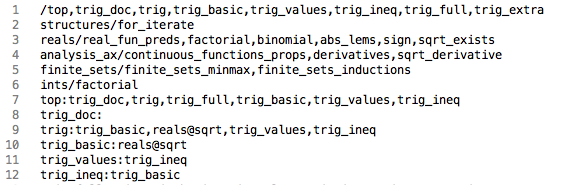
\includegraphics[width=11cm]{images/top.png}
  \caption{Overview of metadata file for package \cde{trig} in NASALib.}
  \label{fig.top}
\end{figure}
